\documentclass[12pt,addpoints]{repaso}
\grado{3}
\nivel{Secundaria}
\cicloescolar{2024-2025}
\materia{Matemáticas}
\unidad{2}
\title{Practica la Unidad}
\aprendizajes{
    \item Usa e interpreta las medidas de tendencia central (moda, media aritmética y mediana) y el rango de un conjunto de datos, y decide cuál de ellas conviene más en el análisis de los datos en cuestión
    \item Formula expresiones de primer grado para representar propiedades (perímetros y áreas) de figuras geométricas y verifica equivalencia de expresiones, tanto algebraica como geométricamente (análisis de las figuras).
    \item Resuelve problemas mediante la formulación y solución algebraica de ecuaciones lineales.
    \item Calcula el área y volumen de piramides, prismas y cilindros rectos.
    }
\author{Melchor Pinto, J.C.}
\begin{document}
\INFO
\begin{multicols}{2}
	\tableofcontents
\end{multicols}
\vfill
\afterpage{\blankpage}
\begin{questions}
    \section{Probabilidad y estadística}
    \subsection{Media, Mediana, Moda y Desviación media}
   
    \questionboxed[2]{Determina la mediana y la moda en los siguientes conjuntos de datos:
      
    \begin{multicols}{2}
            \begin{parts}
                % \part 80, 82, 85, 88, 90, 88, 91, 85, 95, 88, 88, 97, 100. \\[1em]
                % La media es: \fillin[$89$][0.4in]. \\
                % La mediana es: \fillin[$88$][0.4in].\\
                % La moda es: \fillin[$88$][0.4in].  \\

                \part Los puntajes obtenidos en un juego son: \\54, 55, 59, 61, 77, 58, 55, 71, 59, 55, 60, 53, 56 y 60. \\[1em]
                La media es: 
                
                  \begin{solutionbox}{2cm}
                    $\dfrac{54+55+59+\ldots+56+60}{14}=    \dfrac{823}{14}=59.5$
                \end{solutionbox}

                La mediana es: \fillin[$58.5$][0in].\\
                La moda es: \fillin[$55$][0in]. \\
                La desviación media es: %\fillin[$4.5$][0in].

                \begin{solutionbox}{2cm}
                 Para calcular la desviación media:\\
                    \[\dfrac{|54-59.5|+|55-59.5|+\ldots+|60-59.5|}{14}=4.5\]
                \end{solutionbox}
                   
                \part 22, 25, 21, 23, 29, 30, 28, 27, 23, 26. \\[1em]
                La media es: 
                
                \begin{solutionbox}{2cm}
                $\dfrac{22+25+21+\ldots+23+26}{10}=\dfrac{254}{10}=25.4$
                \end{solutionbox}

                La mediana es: \fillin[$25.5$][0in].\\
                La moda es: \fillin[$23$][0in].\\
                La desviación media es: %\fillin[$2.6$][0in].

                \begin{solutionbox}{2cm}
                    Para calcular la desviación media:\\
                    \[\frac{|22-25.4|+|25-25.4|+\ldots+|26-25.4|}{10}=2.6\]
                \end{solutionbox}
                % \part Las estaturas de un grupo de personas son: 170, 168, 169, 171, 168, 172, 168, 171 y 173 cm. \\[1em]
                % La media es: \fillin[$170$][0.4in]. \\
                % La mediana es: \fillin[$170$][0.4in].\\
                % La moda es: \fillin[$168$][0.4in]. \\
            \end{parts}
        \end{multicols}
    }


    \subsection{Eventos mutuamente excluyentes}
  
    \questionboxed[4]{Resuelve los siguientes problemas:
    
    % \begin{multicols}{3}
    \begin{parts}
        % \part En una urna hay 10 pelotas azules, 5 verdes, 15 blancas y 20 negras. Calcula la probabilidad de sacar una pelota negra.

        % \begin{solutionbox}{2cm}
            
        % \end{solutionbox}


        % \part Calcula la probabilidad de que al lanzar un dado caiga un número mayor a 5.

        % \begin{solutionbox}{2cm}
        %     Ya que el dado tiene 6 caras, y sólo hay una de ellas que cumple con la condición, la probabilidad de que caiga un número mayor a 5 es de $\dfrac{1}{6}$.
        % \end{solutionbox}

        \part En un salón hay 24 niñas, de las cuales 8 son extranjeras y 16 son mexicanas y hay 22 niños, de los cuales 18 son mexicanos y 4 son extranjeros. Calcula la probabilidad de elegir a un niño extranjero.
        
        \begin{solutionbox}{2.5cm}
            Para calcular la probabilidad de elegir a un niño extranjero, hay que calcular la probabilidad de elegir a un niño, que es de $\dfrac{22}{46}$ y la probabilidad de elegir a un extranjero, que es de $\dfrac{4}{22}$. Por lo tanto, la probabilidad de elegir a un niño extranjero es de $\dfrac{4}{46}=\dfrac{2}{23}$
            \end{solutionbox}

              \part En una urna hay 8 pelotas moradas, 12 naranjas, 7 rojas, 11 azules y 7 blancas. Calcula la probabilidad de sacar una pelota roja o azul.

        \begin{solutionbox}{2.5cm}
            Para calcular la probabilidad de sacar una pelota roja o azul, hay que calcular la probabilidad de sacar una pelota roja, que es de $\dfrac{7}{45}$ y la probabilidad de sacar una pelota azul, que es de $\dfrac{11}{45}$. Por lo tanto, la probabilidad de sacar una pelota roja o azul es de $\dfrac{7}{45}+\dfrac{11}{45}=\dfrac{18}{45}=\dfrac{2}{5}$
        \end{solutionbox}

        % \part En una urna hay 8 pelotas moradas, 12 naranjas, 7 rojas, 11 azules y 7 blancas. Calcula la probabilidad de sacar una pelota negra.

        % \begin{solutionbox}{2cm}

        % \end{solutionbox}

        % \part Si se lanzan tres monedas al aire, calcula la probabilidad de que caiga puro sol.

        % \begin{solutionbox}{2cm}

        % \end{solutionbox}
    \end{parts}
        % \end{multicols}
    }

    \newpage

    \section{ Figuras y cuerpos geométricos}

    \subsection{Perímetro y Área}
   
    \questionboxed[3]{Encuentra el perímetro y el área de las siguientes figuras:
      
    \begin{multicols}{3}
            \begin{parts}
                \part 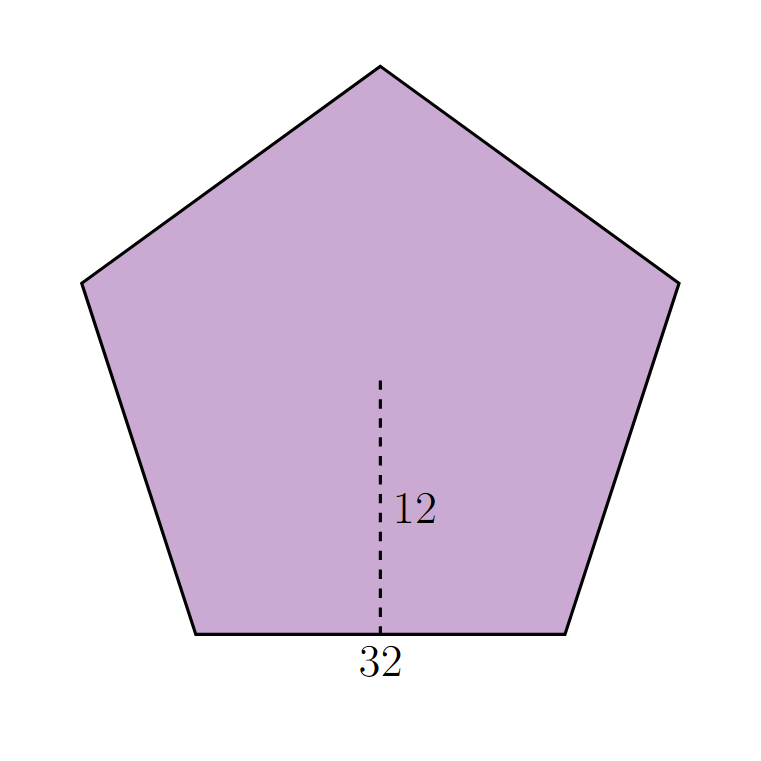
\includegraphics[width=0.9\linewidth]{mex_0018.png} \\
                Perímetro: \fillin[$31\times 3=93$][0in] \\[0.5em] Área: \fillin[$\dfrac{31\times 24}{2}=372$][0in]

                % \part 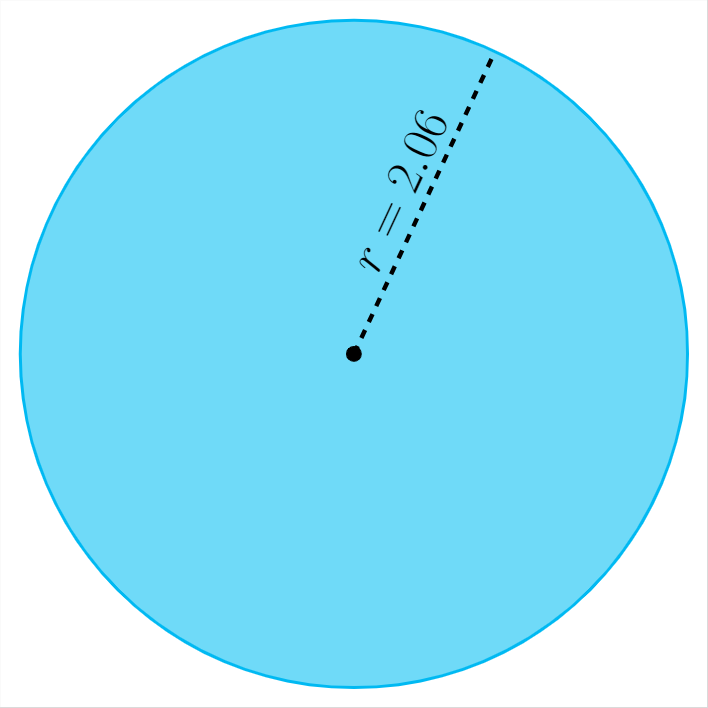
\includegraphics[width=0.9\linewidth]{mex_0001.png} \\
                % Perímetro: \fillin[$11.2 \times 5 = 56$][0in]

                \part 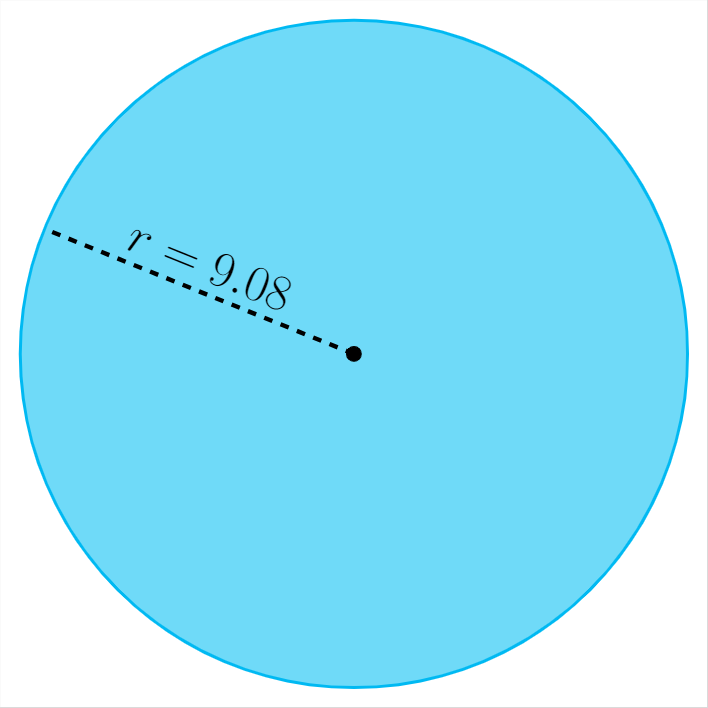
\includegraphics[width=0.9\linewidth]{mex_0012.png} \\
                Perímetro: \fillin[$3.14 \times 88 =276.32$][0in] \\[0.5em]  Área: \fillin[$3.14 \times 44^2 =6079.04$][0in]

                % \part 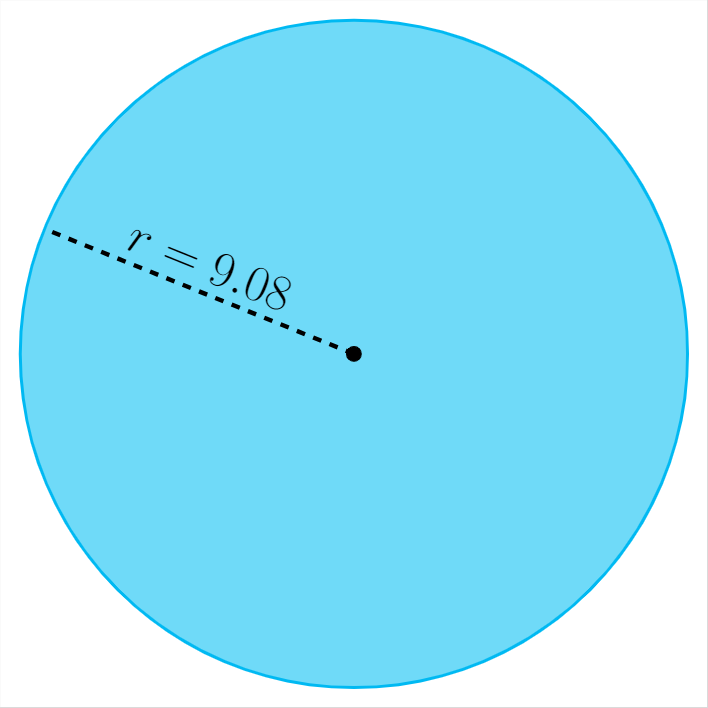
\includegraphics[width=0.9\linewidth]{mex_0013.png}
                % Perímetro: \fillin[$2\times 9.08 \times 3.14=57.02$][0in] \\ Área: \fillin[$3.14 \times 9,08^2 =258.88$][0in]


                \part 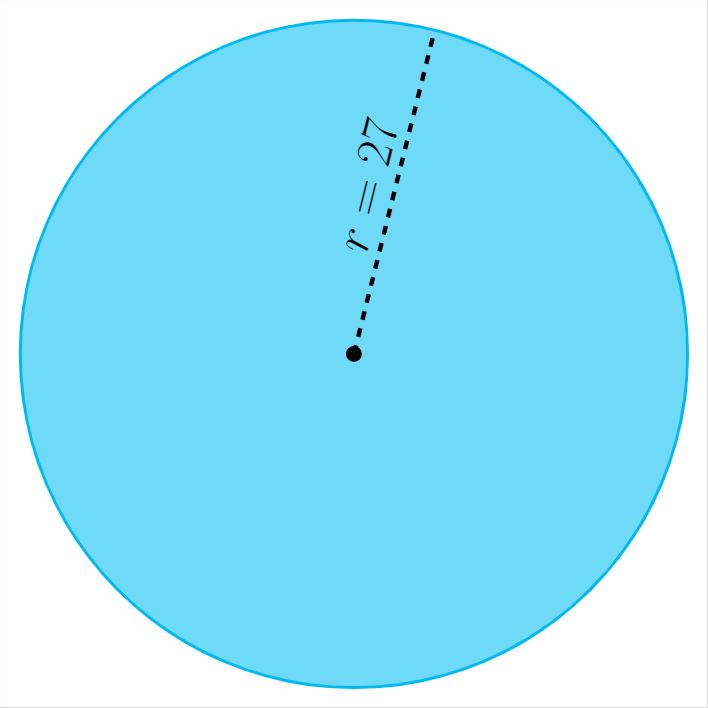
\includegraphics[width=0.9\linewidth]{mex_0006.png}
                Perímetro: \fillin[$2(42.9+21)=127.8$][0in] \\[0.5em]  Área: \fillin[$42.9\times 21=900.9$][0in]

                % \part 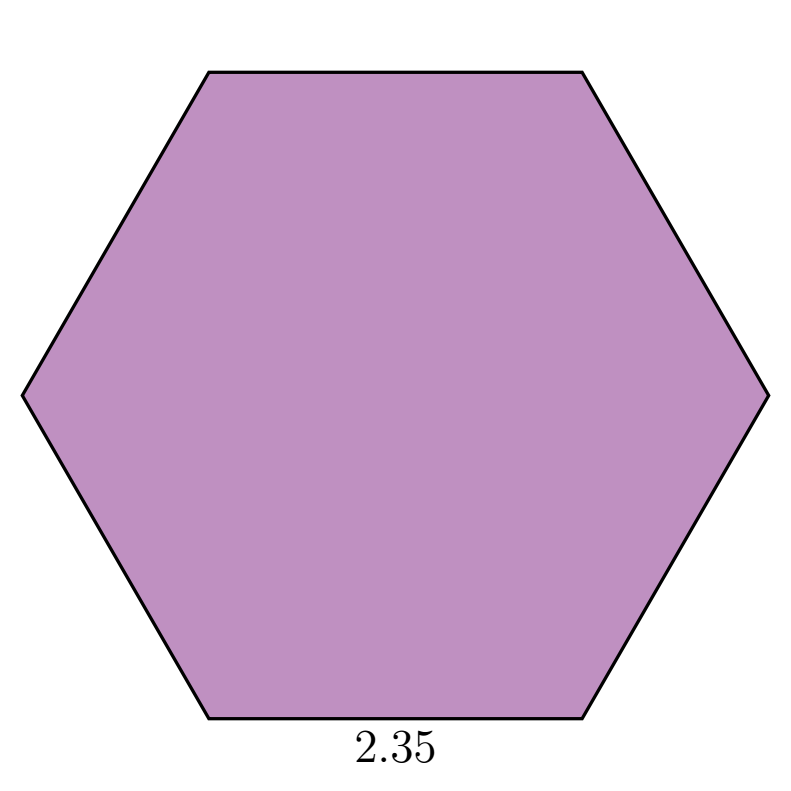
\includegraphics[width=0.9\linewidth]{mex_0007.png}
                % Perímetro: \fillin[$2.35\times 6=14.1$][0in] 

            \end{parts}
        \end{multicols}
    }

    \subsection{Resolución de problemas}
  
    \questionboxed[4]{Resuelve los siguientes problemas:
     
    \begin{multicols}{2}
            \begin{parts}
                \part Calcula la altura de un prisma que tiene como área de la base 6 m$^2$ y 66 m$^3$ de capacidad.

                \begin{solutionbox}{2.5cm}
Ya que el volumen de un prisma es: $V=A_b\cdot h$, entonces la altura del prisma es: \[h=\dfrac{V}{A_b}=\dfrac{66}{6}=11\text{m}\]
                \end{solutionbox}

                \part ¿Cuál es el perímetro de un campo de fútbol que mide 95.12 metros de largo y 45.27 metros de ancho?

                \begin{solutionbox}{3.2cm}
                Ya que el perímetro de un rectángulo es: \[P=2(l+a)\] entonces el perímetro del campo de fútbol es: \[P=2(95.12+45.27)=280.78\text{m}\]
                \end{solutionbox}

                \part Calcula la altura de un prisma que tiene como área de la base 8 m$^2$ y 120 m$^3$ de capacidad.

                \begin{solutionbox}{2.5cm}
Ya que el volumen de un prisma es: $V=A_b\cdot h$, entonces la altura del prisma es: \[h=\dfrac{V}{A_b}=\dfrac{120}{8}=15\text{m}\].
                \end{solutionbox}

                \part Ricardo quiere poner una barda alrededor de un terreno pentagonal que mide 15 metros por lado. ¿Cuánta barda necesitará Ricardo para poner barda en todo el terreno?

                \begin{solutionbox}{2.5cm}
Se sabe que el perímetro de un pentágono es: $P=5l$, entonces el perímetro del terreno es: \[P=5(15)=75\text{m}\]
                \end{solutionbox}
            \end{parts}
        \end{multicols}
    }

    \subsection{Área lateral, Área total y Volumen}
  
    \questionboxed[4]{Calcula el volumen, el área lateral y el área total de las siguientes figuras:
     
    \begin{multicols}{2}
            \begin{parts}
                \part 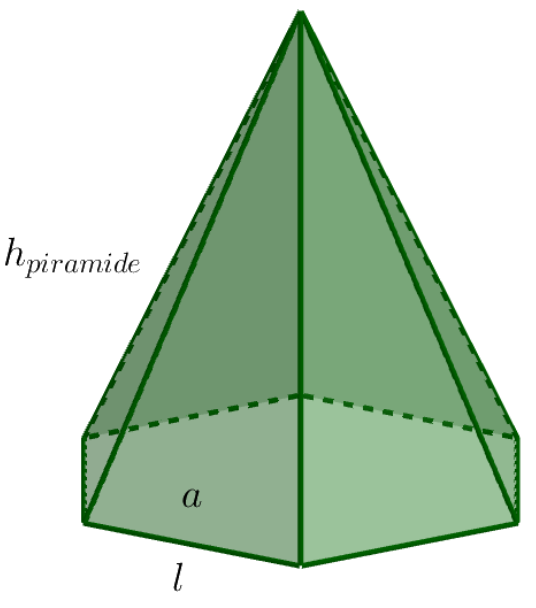
\includegraphics[width=0.5\linewidth]{mex_0022.png} \\
                Pirámide hexagonal cuyos lados "l" de la base miden 8 cm, su apotema mide 7 cm y la altura mide 21 cm.
               
                \begin{solutionbox}{5.5cm}
                   Volumen: 
                    \[V=\dfrac{1}{3}A_b\cdot h= \dfrac{1}{3}\left(\dfrac{nla}{2}\right)h= \dfrac{6(8)7}{6}(21)=1176\]
                A. Lateral:
                    \[A_L=n\dfrac{lh}{2}=6\cdot 8\cdot 21=1008\]
                 A. Total: 
                    \[A_T=A_L+\dfrac{nla}{2}=840+64=904\]
                    \end{solutionbox}

                % \part 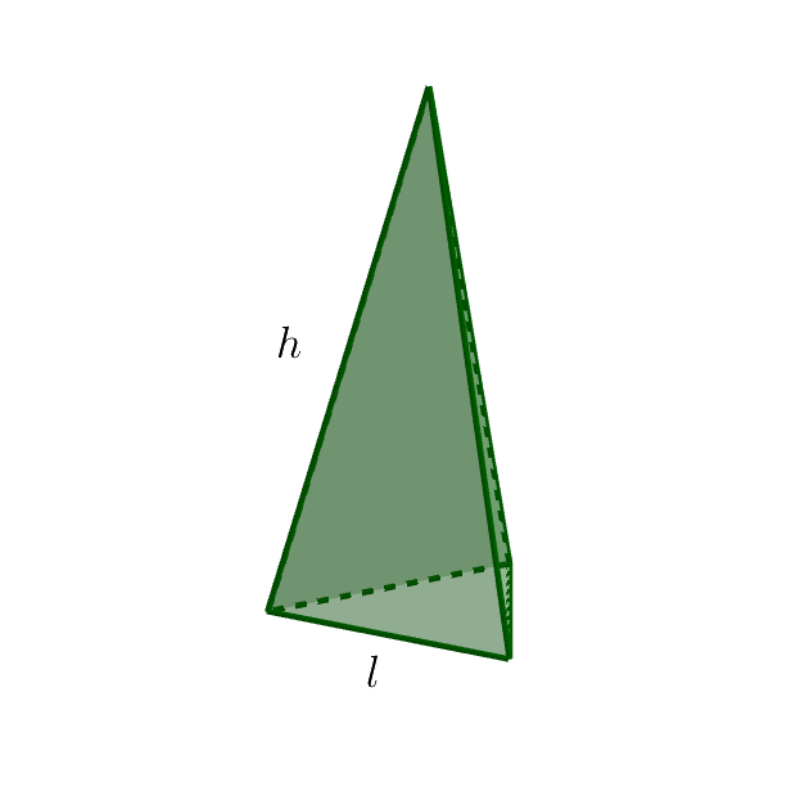
\includegraphics[width=\linewidth]{mex_0023.png}
                % Pirámide cuyos lados "l" de la base miden 13 cm y la altura "h" mide 42 cm.\\
                % Volumen: \fillin[$$ u$^3$][0.4in] \\A. Lateral: \fillin[$$ u][0.4in] \\ A. Total: \fillin[$$ u$^2$][0.4in]

                \part 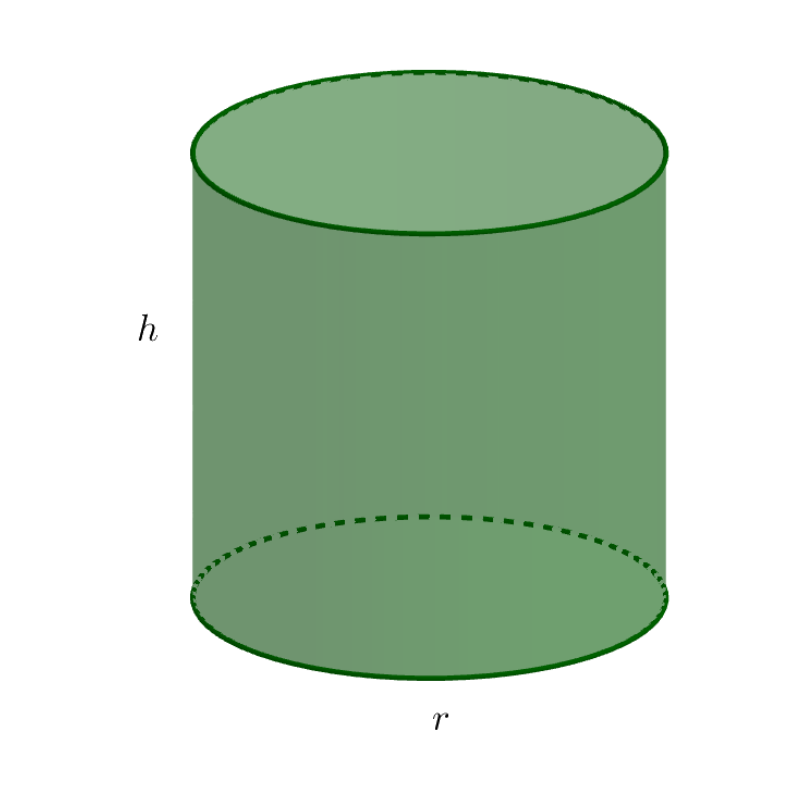
\includegraphics[width=0.5\linewidth]{mex_0024.png} \\
                Cilindro con altura $h=17$ cm y un radio $r=4$ cm.
            
                \begin{solutionbox}{4.5cm}
                    Volumen: 
                    \[V=\pi r^2h=(3.14) 4^2\cdot 17= 857.12\]
                A. Lateral:
                    \[A_L=2\pi rh=2(3.14) 4\cdot 17= 2(3.14) 68=428.48\]
                A. Total: 
                \[A_T=A_L+2\pi r^2=428.48+2(3.14) 16=528.96\]
                \end{solutionbox}

                % \part 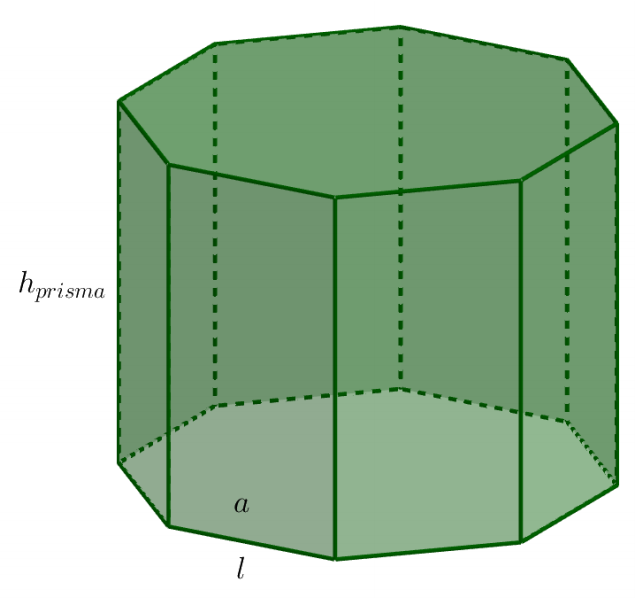
\includegraphics[width=\linewidth]{mex_0025.png}
                % Volumen: \fillin[$$ u$^3$][0.4in] \\A. Lateral: \fillin[$$ u][0.4in] \\ A. Total: \fillin[$$ u$^2$][0.4in]

                % \part 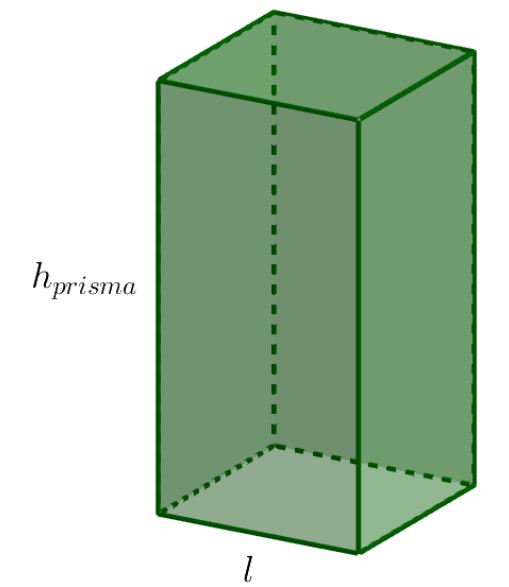
\includegraphics[width=\linewidth]{mex_0026.png}
                % Prisma cuyos lados "l" de la base miden 15 cm y la altura "h" mide 24 cm.\\
                % Volumen: \fillin[$$ u$^3$][0.4in] \\A. Lateral: \fillin[$$ u][0.4in] \\ A. Total: \fillin[$$ u$^2$][0.4in]

                \part 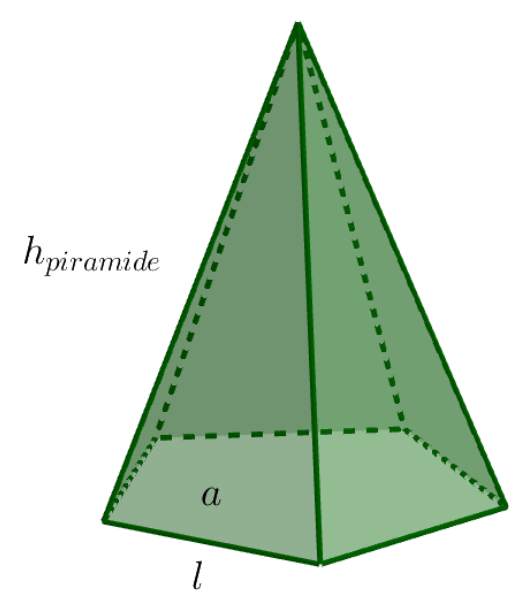
\includegraphics[width=0.5\linewidth]{mex_0027.png} \\
                Pirámide pentagonal de 19 cm de altura cuya base es un pentágono cuyos lados "l" miden 8 cm y su apotema mide 5 cm.
             
                \begin{solutionbox}{5.5cm}
                    Volumen: 
                     \[V=\dfrac{1}{3}A_b\cdot h= \dfrac{1}{3}\left(\dfrac{nla}{2}\right)h= \dfrac{5(8)5}{2}(19)=950\]
                 A. Lateral:
                     \[A_L=n\dfrac{lh}{2}=5\cdot 8\cdot 19=760\]
                  A. Total: 
                     \[A_T=A_L+\dfrac{nla}{2}=760+100=860\]
                     \end{solutionbox}
 

                % \part 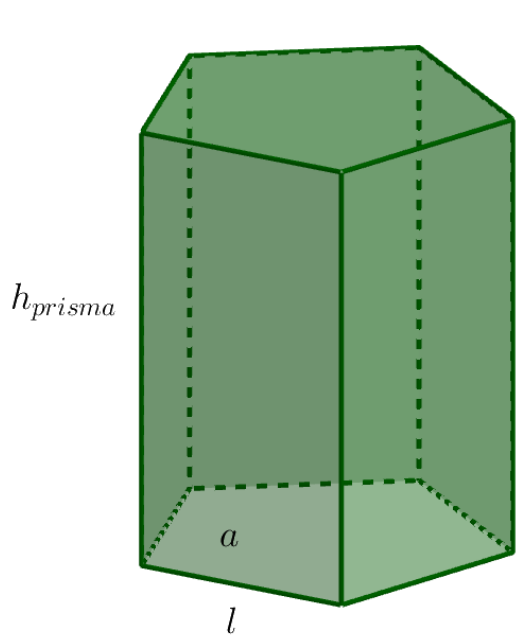
\includegraphics[width=\linewidth]{mex_0028.png}
                % Volumen: \fillin[$$ u$^3$][0.4in] \\A. Lateral: \fillin[$$ u][0.4in] \\ A. Total: \fillin[$$ u$^2$][0.4in]

                \part 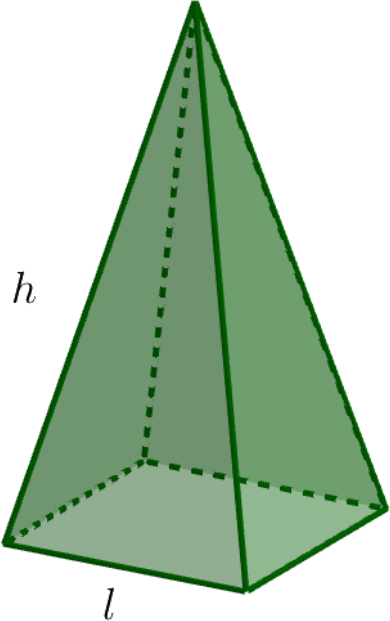
\includegraphics[width=0.5\linewidth]{mex_0029.png} \\
                Pirámide cuadrada cuyos lados "l" de la base miden 16 cm y la altura "h" mide 27 cm.
               
                \begin{solutionbox}{4.5cm}
                    Volumen: 
                     \[V=\dfrac{1}{3}A_b h= \dfrac{1}{3}l^2h= \dfrac{1}{3}16^2(27)=2304\]
                 A. Lateral:
                     \[A_L=n\dfrac{lh}{2}=4\cdot \dfrac{16\times 27}{2}=864\]
                     \[A_T=A_L+l^2=864+16^2=864+256=1120\]
                     \end{solutionbox}
 
                % \part 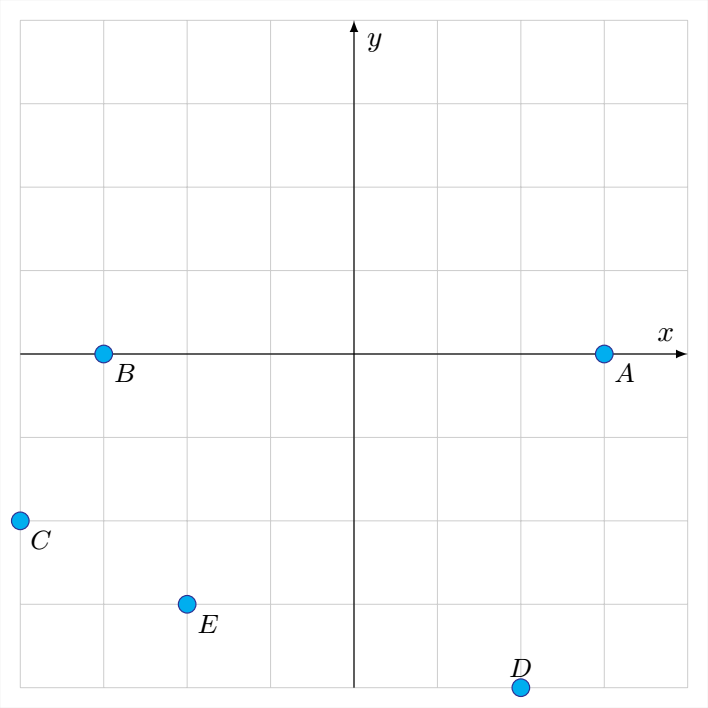
\includegraphics[width=\linewidth]{mex_0030.png}
                % Volumen: \fillin[$$ u$^3$][0.4in] \\A. Lateral: \fillin[$$ u][0.4in] \\ A. Total: \fillin[$$ u$^2$][0.4in]

            \end{parts}
        \end{multicols}
    }

    \section{Plano cartesiano y recta}

    \subsection{Ubicación en el plano cartesiano}

    \questionboxed[10]{ Observa la siguiente figura e indica las coordenadas y el cuadrante para cada uno de los puntos:
      
    \begin{minipage}[t]{0.45\linewidth}
            \begin{figure}[H]
                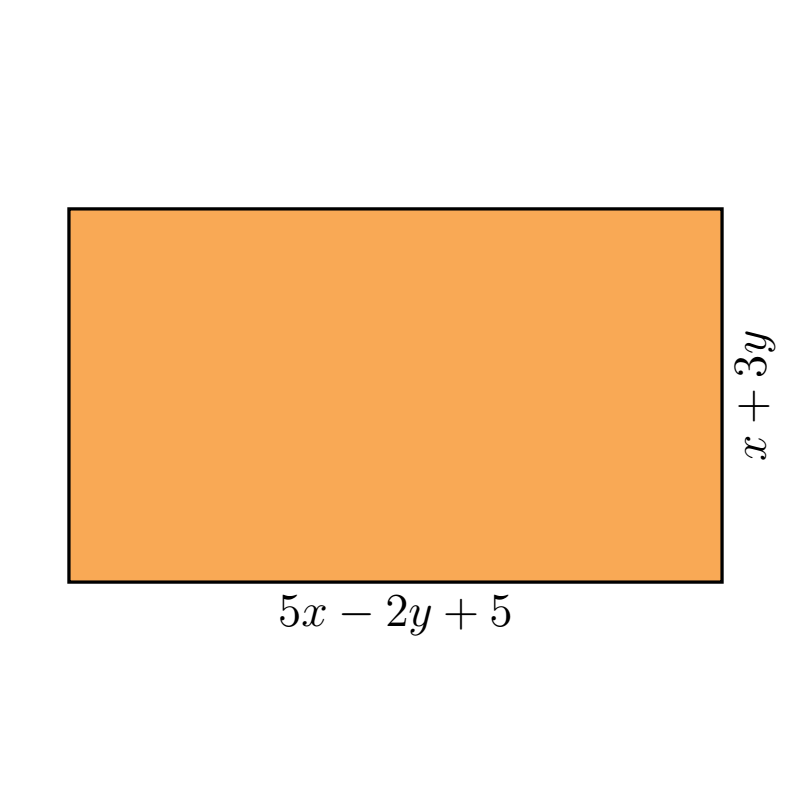
\includegraphics[width=\linewidth]{mex_0031.png}
            \end{figure}
        \end{minipage}\hfill
        \begin{minipage}[t]{0.5\linewidth}
            \begin{parts}
                \part Coordenadas del punto A \fillin[$(1,5)$][0.5in]
               
                \begin{oneparchoices}\small%
                \choice Eje $x$
                \choice Eje $y$
                \CorrectChoice Cuad. I 
                \choice Cuad. II \\
                \choice Cuad. III
                \choice Cuad. IV
            \end{oneparchoices}
            
            \part Coordenadas del punto B \fillin[$(-3,6)$][0.5in]
              
                \begin{oneparchoices}\small%
                \choice Eje $x$
                \choice Eje $y$
                \choice Cuad. I 
                \CorrectChoice Cuad. II \\
                \choice Cuad. III
                \choice Cuad. IV
            \end{oneparchoices}
            
            \part Coordenadas del punto C \fillin[$(5,-3)$][0.5in]
               
                \begin{oneparchoices}\small%
                \choice Eje $x$
                \choice Eje $y$
                \choice Cuad. I 
                \choice Cuad. II \\
                \choice Cuad. III
                \CorrectChoice Cuad. IV
            \end{oneparchoices}
              
            \part Coordenadas del punto D \fillin[$(-5,0)$][0.5in]
                
                \begin{oneparchoices}\small%
                \CorrectChoice Eje $x$
                \choice Eje $y$
                \choice Cuad. I 
                \choice Cuad. II \\
                \choice Cuad. III
                \choice Cuad. IV
            \end{oneparchoices}

                \part Coordenadas del punto E \fillin[$(0,-7)$][0.5in]
          
                \begin{oneparchoices}\small%
                \choice Eje $x$
                \CorrectChoice Eje $y$
                \choice Cuad. I 
                \choice Cuad. II \\
                \choice Cuad. III
                \choice Cuad. IV
            \end{oneparchoices}
            \end{parts}
        \end{minipage}
    }

   

    \subsection{Cuadrantes en el plano cartesiano}
 
    \questionboxed[6]{Selecciona la respuesta correcta:
      
    \begin{multicols}{2}
            \begin{parts}
                \part El punto A$(0,8.24)$, ¿está ubicado sobre el eje $y$?

                \begin{oneparcheckboxes}
                    \CorrectChoice Verdadero
                    \choice Falso
                \end{oneparcheckboxes}

                \part El punto A$(0,-10)$, ¿está ubicado sobre el eje $x$?

                \begin{oneparcheckboxes}
                    \choice Verdadero
                    \CorrectChoice Falso
                \end{oneparcheckboxes}

                \part El punto A$(2,0)$, ¿está ubicado sobre el eje $y$?

                \begin{oneparcheckboxes}
                    \choice Verdadero
                    \CorrectChoice Falso
                \end{oneparcheckboxes}

                \part El punto A$(0,-5.19)$, ¿está ubicado sobre el eje $x$?

                \begin{oneparcheckboxes}
                    \choice Verdadero
                    \CorrectChoice Falso
                \end{oneparcheckboxes}

                \part El punto A$(-1.5,0)$, ¿está ubicado sobre el eje $x$?

                \begin{oneparcheckboxes}
                    \CorrectChoice Verdadero
                    \choice Falso
                \end{oneparcheckboxes}

                \part El punto A$(1,0)$, ¿está ubicado sobre el eje $x$?

                \begin{oneparcheckboxes}
                    \CorrectChoice Verdadero
                    \choice Falso
                \end{oneparcheckboxes}
            \end{parts}
        \end{multicols}
    }

    \subsection{Ecuación de una recta}
    
    \questionboxed[3]{Escribe la ecuación de las recta para dada uno de los siguientes incisos:
    
    \begin{parts}
            \part Escribe la ecuación de la recta que pasa por los puntos $A(3,-2)$ y $B(4,6)$.

            \begin{solutionbox}{2.5cm}\footnotesize%
                Para obtener la ecuación necesitamos calcular la pendiente de la recta, que es: \[m=\dfrac{y_2-y_1}{x_2-x_1}=\dfrac{6-(-2)}{4-3}=\dfrac{8}{1}=8\], y la ordenada al origen, que es: $b=y-mx=-2-8(3)=-2-24=-26$. \\
                Por lo tanto, la ecuación de la recta es: $y=8x-26$.
            \end{solutionbox}

            \part Escribe la ecuación de la recta que pasa por los puntos$ A(1,6)$ y $B(2,1)$
           
            \begin{solutionbox}{2.5cm}\footnotesize%
                Para obtener la ecuación necesitamos calcular la pendiente de la recta, que es: \[m=\dfrac{y_2-y_1}{x_2-x_1}= \dfrac{1-6}{2-1}=\dfrac{-5}{1}=-5\], y la ordenada al origen, que es: $b=y-mx=6-5(1)=6-5=1$. \\
                Por lo tanto, la ecuación de la recta es: $y=-5x+1$.
            \end{solutionbox}

            \part Escribe la ecuación de la recta que pasa por los puntos $A(-2,3)$ y $B(1,0)$

            \begin{solutionbox}{2.5cm}\footnotesize%
                Para obtener la ecuación necesitamos calcular la pendiente de la recta, que es: \[m=\dfrac{y_2-y_1}{x_2-x_1}= \dfrac{0-3}{1-(-2)}=\dfrac{-3}{3}=-1\], y la ordenada al origen, que es: $b=y-mx=3-(-1)(-2)=3+2=5$. \\
                Por lo tanto, la ecuación de la recta es: $y=-x+5$.
            \end{solutionbox}
        \end{parts}
    }

   
    \subsection{Pendiente y ordenada}
    
    \questionboxed[5]{Identifica la pendiente y ordenada de las siguientes rectas:
      
    \begin{parts}
            \begin{multicols}{3}
                \part $y=-2x+1$ \\[1em]
                Pendiente = \fillin[$-2$][0in]  \\ Ordenada = \fillin[$1$][0in]

                \part $y=\frac{1}{2}x-3$ \\[1em]
                Pendiente = \fillin[$\frac{1}{2}$][0in]  \\ Ordenada = \fillin[$-3$][0in]

                \part $y=-3x+3$ \\[1em]
                Pendiente = \fillin[$-3$][0in]  \\ Ordenada = \fillin[$3$][0in]
            \end{multicols}

            \begin{multicols}{2}
                \part 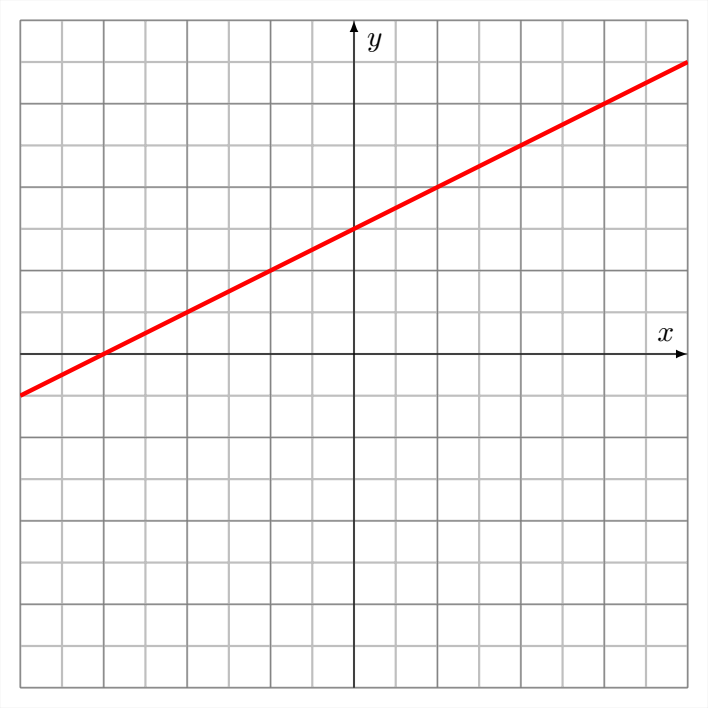
\includegraphics[width=0.5\linewidth]{mex_0047.png}\\
                Pendiente = \fillin[$\dfrac{1}{2}$][0in] \qquad \qquad Ordenada = \fillin[$3$][0in]

                \part 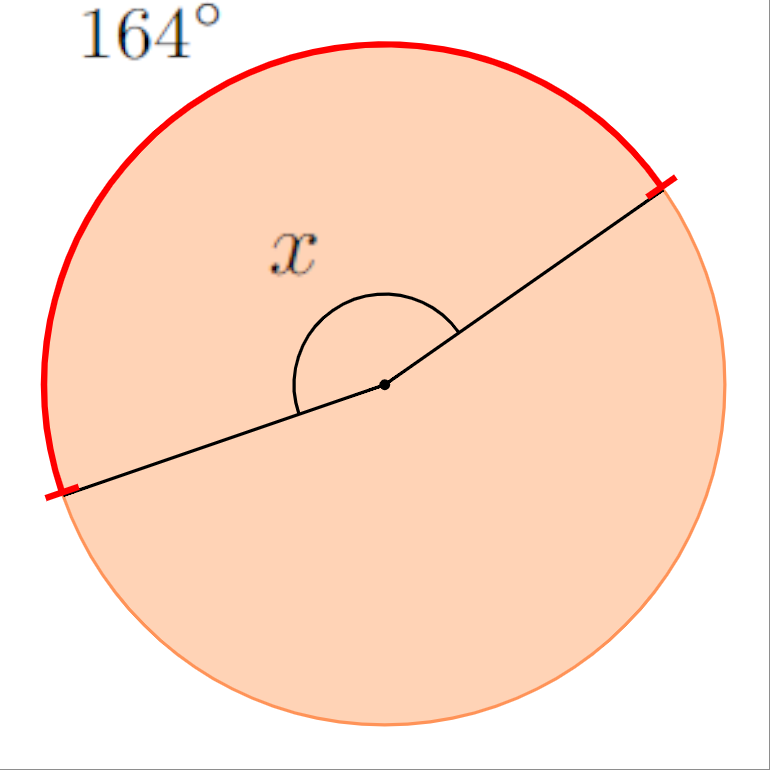
\includegraphics[width=0.5\linewidth]{mex_0051.png}\\
                Pendiente = \fillin[$-2$][0in]  \qquad \qquad Ordenada = \fillin[$0$][0in]
            \end{multicols}

        \end{parts}
    }



    \subsection{Pendiente dados dos puntos}
  
    \questionboxed[7]{Calcula la pendiente en cada uno de los siguientes incisos:
     
    \begin{multicols}{2}
            \begin{parts}
                \part Calcula la pendiente de la recta que pasa por los puntos A(0,-3) y B(5,1).   \\[1em]
                $m=$ \fillin[$\dfrac{4}{5}$][0in]
                \part Calcula la pendiente de la recta que pasa por los puntos A(-8,6) y B(-3,8).  \\[1em]
                $m=$ \fillin[$\dfrac{2}{5}$][0in]
                \part Calcula la pendiente de la recta que pasa por los puntos A(1,1) y B(5,-3).   \\[1em]
                $m=$ \fillin[$-1$][0in]
                \part Calcula la pendiente de la recta que pasa por los puntos A(-7,-3) y B(6,10). \\[1em]
                $m=$ \fillin[$1$][0in]
                \part Calcula la pendiente de la recta que pasa por los puntos A(-7,-3) y B(-5,7). \\[1em]
                $m=$ \fillin[$5$][0in]

                \columnbreak%

                \part Calcula la pendiente de la siguiente recta:\\
                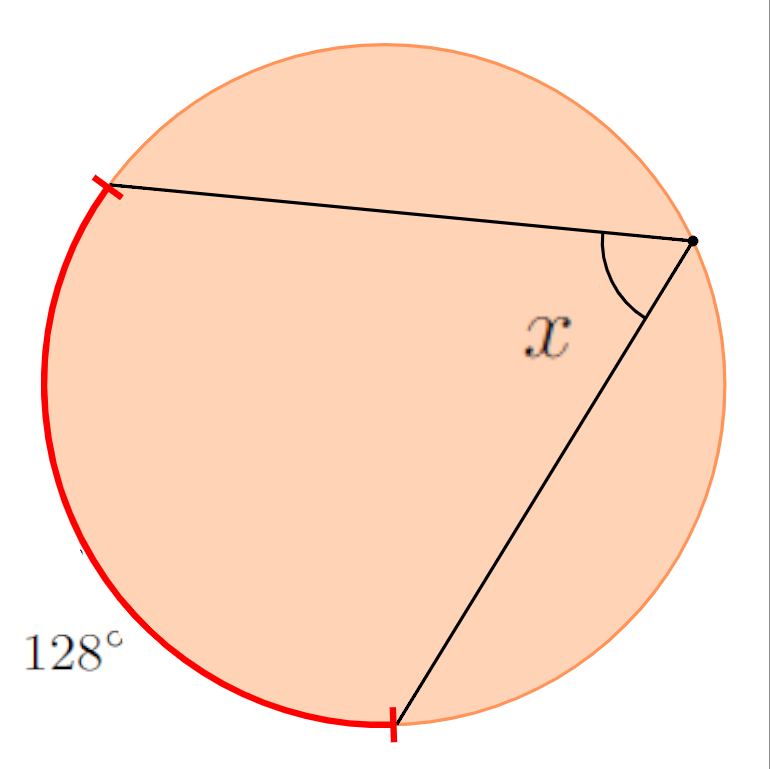
\includegraphics[width=0.6\linewidth]{mex_0050.png} $m=$ \fillin[$-1$][0in]

                \part Calcula la pendiente de la siguiente recta:\\
                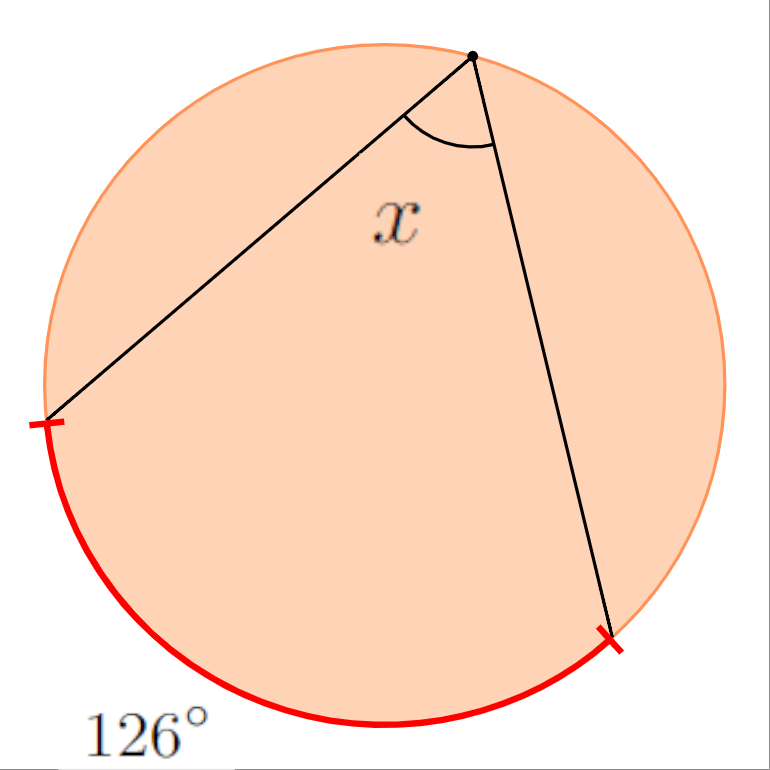
\includegraphics[width=0.6\linewidth]{mex_0048.png} $m=$ \fillin[$-\dfrac{1}{2}$][0in]
            \end{parts}
        \end{multicols}
    }

    \section{Ecuación lineal}

    \subsection{Ecuaciones lineales}
  
    \questionboxed[3]{Resuelve las siguientes ecuaciones lineales
       
    \begin{multicols}{3}
            \begin{parts}
                % \part $2x=-30$         \fillin[$x=-15$][0in]            \\
                % \part $x-23=-36$       \fillin[$x=-13$][0in]            \\
                % \part $-4x=-6$         \fillin[$x=\dfrac{3}{2}$][0in]   \\
                % \part $6x=-36$         \fillin[$x=-6$][0in]             \\
                \part $6x-2=10$      %  \fillin[$x=2$][0in]
                
                \begin{solutionbox}{3.8cm}
                \[6x-2=10\] \[6x=10+2\] \[6x=12\] \[x=\dfrac{12}{6}\] \[x=2\]
                \end{solutionbox}

                % \part $12x-36=-60$     \fillin[$x=-2$][0in]           \\
                % \part $-4x+1=2x+7$     \fillin[$x=-1$][0in]           \\
                \part $9x-8=5x+4$     % \fillin[$x=3$][0in]

                \begin{solutionbox}{3.8cm}
                    \[9x-8=5x+4\] \[9x-5x=4+8\] \[4x=12\] \[x=\dfrac{12}{4}\] \[x=3\]
                \end{solutionbox}
                % \part $5(-3x+5)=20$    \fillin[$x=\dfrac{1}{3}$][0in] \\

                \part $32x+24=5(2x-4)$ %\fillin[$x=-2$][0in]

                \begin{solutionbox}{3.8cm}
                    \[32x+24=5(2x-4)\] \[32x+24=10x-20\] \[32x-10x=-20-24\] \[22x=-44\] \[x=-2\]
                \end{solutionbox}
            \end{parts}
        \end{multicols}
    }

    \subsection{Lenguaje algebraico}
   
    \questionboxed[8]{Escribe la expresión algebraica correcta para los siguientes enunciados
       
    \begin{multicols}{2}
            \begin{parts}
                \part La cuarta parte de un número cualquiera.
                   \fillin[$\frac{x}{4}$ o $\frac{1}{4}x$][0in]

                \part El cuadrado de la diferencia de dos números cualquiera.
                    \fillin[$(x-y)^2$][0in]

                \part El cubo de un número cualquiera aumentado en 10.
                   \fillin[ $x^3+10$][0in]

                \part El cuadrado de la suma de dos números cualquiera.
                   \fillin[ $(x+y)^2$][0in]

                \part El recíproco de un número cualquiera.
                   \fillin[ $\frac{1}{x}$][0in]

                \part El triple de un número cualquiera.
                    \fillin[$3x$][0in]

                \part La mitad del cubo de la suma de dos números cualquiera.
                    \fillin[$\frac{1}{2}(x+y)^3$][0in]

                \part Dos novenas partes de un número cualquiera.
                    \fillin[$\frac{2}{9}x$][0in]
            \end{parts}
        \end{multicols}
    }


    \subsection{Resolución de problemas}
    
    \questionboxed[6]{Resuelve los siguientes problemas de ecuaciones lineales
     
    \begin{multicols}{2}
    \begin{parts}
            \part La suma de tres números consecutivos es 195. Halla estos números
       
            \begin{solutionbox}{3cm}
                \[x+(x+1)+(x+2)=195\] \[3x+3=195\] \[3x=192\] \[x=64\] 
            \end{solutionbox}
        
            \part La suma de dos números es 215 y el mayor excede al menor en 31 unidades. ¿Cuáles son estos dos números?
           
            \begin{solutionbox}{3cm}
               \[x+(x+31)=215\] \[2x+31=215\] \[2x=184\] \[x=92\] 
            \end{solutionbox}
        \end{parts}
\end{multicols}
    }

    \subsection{Ecuaciones lineales con fracciones}
   
    \questionboxed[10]{Resuelve las siguientes ecuaciones lineales con fracciones

        \begin{multicols}{2}
            \begin{parts}
                \part $-\dfrac{1}{2}x-\dfrac{1}{4}x=\dfrac{5}{6}$

                \begin{solutionbox}{3.2cm}\footnotesize%
                \[ -\frac{2}{4}x-\frac{1}{4}x=\frac{5}{6} \] \[ -\frac{3}{4}x=\frac{5}{6} \] \[ x=\frac{5}{6}\divisionsymbol -\frac{3}{4} \]  \[ x=-\frac{10}{9} \]
                \end{solutionbox}

                \part $-\dfrac{x}{6}=\dfrac{7}{54}$

                \begin{solutionbox}{3.2cm}\footnotesize%
                    \[ -\frac{x}{6}=\frac{7}{54} \] \[ -\frac{54}{6}x=7 \] \[ -9x=7 \]  \[ x=-\frac{7}{9} \]
                \end{solutionbox}
            \end{parts}
        \end{multicols}
    }

    \section{Sistemas de ecuaciones}
        % \subsection{{Método de sustitución e igualación}

    % \questionboxed[15]{Numera correctamente los pasos para resolver un sistema de dos ecuaciones con dos inc\'ognitas por los m'etodos a continuaci\'on:
    %     \begin{choices}
    %         \choice M\'etodo de sustitución:
    %         \begin{itemize}
    %             \item[\rule{1cm}{0.2mm}] Despejar una inc\'ognita en una de las ecuaciones.
    %             \item[\rule{1cm}{0.2mm}] Resolver la ecuaci\'on resultante.
    %             \item[\rule{1cm}{0.2mm}] Sustituir el valor obtenido en la ecuaci\'on en la que aparec\'ia la inc\'ognita despejada.
    %             \item[\rule{1cm}{0.2mm}] Sustituir la expresi\'on de esta inc\'ognita en la otra ecuaci\'on para obtener una ecuaci\'on con una sola inc\'ognita.
    %             \item[\rule{1cm}{0.2mm}] Sustituir los valores en las ecuaciones originales para comprobar que son la soluci\'on.
    %         \end{itemize}

    %         \choice M\'etodo de suma-resta:
    %         \begin{itemize}
    %             \item[\rule{1cm}{0.2mm}] Resolver la ecuaci\'on resultante.
    %             \item[\rule{1cm}{0.2mm}] Sumar o restar las ecuaciones para eliminar una de las inc\'ognitas.
    %             \item[\rule{1cm}{0.2mm}] Sustituir los valores en las ecuaciones originales para comprobar que son la soluci\'on.
    %             \item[\rule{1cm}{0.2mm}] Multiplicar una o ambas ecuaciones por los n\'umeros necesarios para realizar la eliminaci\'on bajo la suma o resta.
    %             \item[\rule{1cm}{0.2mm}] Sustituir el valor obtenido en una de las ecuaciones iniciales y resolverla.
    %         \end{itemize}


    %         \choice M\'etodo de igualaci\'on:
    %         \begin{itemize}
    %             \item[\rule{1cm}{0.2mm}] Resolver la ecuaci\'on resultante.
    %             \item[\rule{1cm}{0.2mm}] Despejar la misma inc\'ognita en ambas ecuaciones.
    %             \item[\rule{1cm}{0.2mm}] Sustituir los valores en las ecuaciones originales para comprobar que son la soluci\'on.
    %             \item[\rule{1cm}{0.2mm}] Igualar las expresiones para obtener una ecuaci\'on con una inc\'ognita
    %             \item[\rule{1cm}{0.2mm}] Sustituir el valor obtenido en cualquiera de las dos expresiones en las que aparec\'ia despejada la otra inc\'ognita.
    %         \end{itemize}
    %     \end{choices}
    % }

    \subsection{Método de eliminación}

    \questionboxed[10]{Utilizando el m\'etodo de eliminación, encuentra el valor de $x$ y $y$ para
        cada uno de los siguientes sistemas de ecuaciones lineales:
       
        \begin{multicols}{2}
            \begin{parts}
                \part
                \begin{eqnarray}
                    2x-y & = & 3 \\
                    3x-y & = & 3 
                \end{eqnarray}

                \setcounter{equation}{0}

                \begin{solutionbox}{8cm}
                    Usando el método de eliminación, multiplicamos la ecuación (1)| por -1 para obtener  $x$:
                    \begin{eqnarray}
                        -2x+y & = & -3 \nonumber\\
                        3x-y & = & 3 \nonumber
                    \end{eqnarray}
                    Sumamos las ecuaciones (2) y (3) para obtener $x$:
                    \begin{eqnarray}
                        x & = & 0 \nonumber
                    \end{eqnarray}
                    Sustituimos el valor de $x$ en la ecuación (1) para obtener $y$:
                    \begin{eqnarray}
                        2(0)-y & = & 3 \nonumber\\
                        -y & = & 3 \nonumber\\
                        y & = & -3 \nonumber 
                    \end{eqnarray}
                \end{solutionbox}

                \part
                \begin{eqnarray}
                    13x-6y & = & 22 \\
                    x & = & y+6 
                \end{eqnarray}

                \setcounter{equation}{0}

                \begin{solutionbox}{7cm}
                    Usando el método de sustitución, sustituimos la ecuación (4) en la ecuación (5) para obtener $x$:
                    \begin{eqnarray}
                        13(y+6)-6y & = & 22 \nonumber\\
                        13y+78-6y & = & 22 \nonumber\\
                        7y & = & -56 \nonumber\\
                        y & = & -8 \nonumber
                    \end{eqnarray}
                    Sustituimos el valor de $y$ en la ecuación (5) para obtener $x$:
                    \begin{eqnarray}
                        x & = & -8+6 \nonumber\\
                        x & = & -2 \nonumber
                    \end{eqnarray}
                \end{solutionbox}
                % \vspace{4cm}
            \end{parts}
        \end{multicols}
    }
 
    % 
    \subsection{Sistema de ecuaciones 3x3}

    \questionboxed[10]{Resuelve el siguiente sistema de ecuaciones lineales:

        \begin{eqnarray}
            x + 2y +3z  & = & 12 \\
            x - 3y +4z  & = & 27 \\
            -x +  y +2z & = & 7 
        \end{eqnarray}

        \begin{solutionbox}{18cm}
            Para resolver el sistema de ecuaciones lineales, sumamos las ecuaciones (1) y (3) para eliminar a $x$ y obtener una ecuación (4):
            \begin{eqnarray}
                x + 2y +3z  & = & 12 \nonumber\\
                -x +  y +2z & = & 7 \nonumber\\ \hline
                3y + 5z & = & 19 
            \end{eqnarray}

            Después, se suman las ecuaciones (2) y (3) para obtener una ecuación (5).

            \begin{eqnarray}
                x - 3y +4z  & = & 27 \nonumber\\
                -x +  y +2z & = & 7 \nonumber\\ \hline
                -2y + 6z & = & 34 
            \end{eqnarray}

            Ahora se resuelve el sistema conformado por las ecuaiones (4) y (5). Para ello multiplicamos la ecuación (4) por 2 y la ecuación (5) por 3 para eliminar a $y$:

            \begin{eqnarray}
                3y + 5z & = & 19 \nonumber\\
                -2y + 6z & = & 34 \nonumber \\ \hline
               6y + 10z & = & 38 \nonumber\\
                -6y + 18z & = & 102 \nonumber \\ \hline
                28z & = & 140 \nonumber\\
                z & = & 5 \nonumber
            \end{eqnarray}
            
            Sustituimos el valor de $z$ en la ecuación (5) para obtener el valor de $z$:

            \begin{eqnarray}
                -2y + 6(5) & = & 34 \nonumber\\
                -2y + 30 & = & 34 \nonumber\\
                -2y & = & 4 \nonumber\\
                y & = & -2 \nonumber
            \end{eqnarray}

            Finalmente, sustituimos los valores de $y$ y $z$ en la ecuación (1) para obtener el valor de $x$:

            \begin{eqnarray}
                x + 2(-2) + 3(5) & = & 12 \nonumber\\
                x - 4 + 15 & = & 12 \nonumber\\
                x + 11 & = & 12 \nonumber\\
                x & = & 1 \nonumber
            \end{eqnarray}
        \end{solutionbox}
    }

    \subsection{Sistema de ecuaciones con fracciones}
  
    \questionboxed[5]{Resuelve el siguiente sistema de ecuaciones lineales con fracciones:
    
    \setcounter{equation}{0}

        \begin{eqnarray}
            12x + 5y                      & = & -6 \\
            \dfrac{5}{3}x - \dfrac{7}{6}y & = & -12    
        \end{eqnarray}

        \begin{solutionbox}{11.5cm}
            Para resolver el sistema de ecuaciones lineales, multiplicamos la ecuación (1) por 7/6 y la ecuación (2) por 5 para eliminar a $y$ y obtener la variable $x$:
           
            \begin{eqnarray}
                14x + \dfrac{35}{6}y & = & -7 \nonumber\\
                \dfrac{25}{3}x - \dfrac{35}{6}y & = & -60 \nonumber
            \end{eqnarray}

            Sumamos las ecuaciones (1) y (2) para obtener $x$:

            \begin{eqnarray}
                14x + \dfrac{35}{6}y & = & -7 \nonumber\\
                \dfrac{25}{3}x - \dfrac{35}{6}y & = & -60 \nonumber\\ \hline
                \dfrac{67}{3}x & = & -67 \nonumber\\
                x & = & -3 \nonumber
            \end{eqnarray}

            Sustituimos el valor de $x$ en la ecuación (1) para obtener $y$:

            \begin{eqnarray}
                12(-3) + 5y & = & -6 \nonumber\\
                -36 + 5y & = & -6 \nonumber\\
                5y & = & 30 \nonumber\\
                y & = & 6 \nonumber
            \end{eqnarray}
        \end{solutionbox}
    }

    % \subsection{{Resolución de problemas}
\end{questions}
\end{document}